% Options for packages loaded elsewhere
\PassOptionsToPackage{unicode}{hyperref}
\PassOptionsToPackage{hyphens}{url}
%
\documentclass[
]{article}
\usepackage{amsmath,amssymb}
\usepackage{iftex}
\ifPDFTeX
  \usepackage[T1]{fontenc}
  \usepackage[utf8]{inputenc}
  \usepackage{textcomp} % provide euro and other symbols
\else % if luatex or xetex
  \usepackage{unicode-math} % this also loads fontspec
  \defaultfontfeatures{Scale=MatchLowercase}
  \defaultfontfeatures[\rmfamily]{Ligatures=TeX,Scale=1}
\fi
\usepackage{lmodern}
\ifPDFTeX\else
  % xetex/luatex font selection
\fi
% Use upquote if available, for straight quotes in verbatim environments
\IfFileExists{upquote.sty}{\usepackage{upquote}}{}
\IfFileExists{microtype.sty}{% use microtype if available
  \usepackage[]{microtype}
  \UseMicrotypeSet[protrusion]{basicmath} % disable protrusion for tt fonts
}{}
\makeatletter
\@ifundefined{KOMAClassName}{% if non-KOMA class
  \IfFileExists{parskip.sty}{%
    \usepackage{parskip}
  }{% else
    \setlength{\parindent}{0pt}
    \setlength{\parskip}{6pt plus 2pt minus 1pt}}
}{% if KOMA class
  \KOMAoptions{parskip=half}}
\makeatother
\usepackage{xcolor}
\usepackage[margin=1in]{geometry}
\usepackage{graphicx}
\makeatletter
\def\maxwidth{\ifdim\Gin@nat@width>\linewidth\linewidth\else\Gin@nat@width\fi}
\def\maxheight{\ifdim\Gin@nat@height>\textheight\textheight\else\Gin@nat@height\fi}
\makeatother
% Scale images if necessary, so that they will not overflow the page
% margins by default, and it is still possible to overwrite the defaults
% using explicit options in \includegraphics[width, height, ...]{}
\setkeys{Gin}{width=\maxwidth,height=\maxheight,keepaspectratio}
% Set default figure placement to htbp
\makeatletter
\def\fps@figure{htbp}
\makeatother
\setlength{\emergencystretch}{3em} % prevent overfull lines
\providecommand{\tightlist}{%
  \setlength{\itemsep}{0pt}\setlength{\parskip}{0pt}}
\setcounter{secnumdepth}{-\maxdimen} % remove section numbering
\usepackage{float}
\usepackage{wrapfig}
\usepackage{caption}
\captionsetup{font=small}
\usepackage{graphicx}
\usepackage{titlesec}
\titlespacing\section{0pt}{12pt plus 4pt minus 2pt}{-5pt plus 2pt minus 2pt}
\ifLuaTeX
  \usepackage{selnolig}  % disable illegal ligatures
\fi
\usepackage{bookmark}
\IfFileExists{xurl.sty}{\usepackage{xurl}}{} % add URL line breaks if available
\urlstyle{same}
\hypersetup{
  pdftitle={High Performance Computing - Exercise 2c},
  pdfauthor={Andrea Buscema},
  hidelinks,
  pdfcreator={LaTeX via pandoc}}

\title{High Performance Computing - Exercise 2c}
\usepackage{etoolbox}
\makeatletter
\providecommand{\subtitle}[1]{% add subtitle to \maketitle
  \apptocmd{\@title}{\par {\large #1 \par}}{}{}
}
\makeatother
\subtitle{Mandelbrot Set - Parallel Computing using MPI + OpenMP}
\author{Andrea Buscema}
\date{30/05/2024}

\begin{document}
\maketitle

\subsection{Introduction}\label{introduction}

In this report, will be discussed the results of the second exercise of
the High Performance Computing assignment. The objective of this
exercise is to implement the Mandelbrot Set using MPI and OpenMP,
obtaining a single pgm image as output, and analysing the scalability of
the implementation:

\begin{itemize}
\tightlist
\item
  OMP scaling: run with a single MPI task and increase the number of OMP
  threads;
\item
  MPI scaling: run with a single OMP thread per MPI task and increase
  the number of MPI tasks;
\item
  Hybrid scaling (such an extra analysis - not required for the
  assignment): run for different combinations of MPI and OMP threads.
\end{itemize}

As for the first exercise/assignment, the project was implemented to be
used in the ORFEO HPC Cluster, using THIN nodes. The project was
implemented in C language, using the MPI and OpenMP libraries, SLURM for
job submission (file .sbatch), and Python for data analysis and
plotting.

\subsubsection{Replication of the
project}\label{replication-of-the-project}

Since the ORFEO Cluster is not available for external users, the project
can be replicated in a local machine or in another cluster and be
represented considering a general usage for most of the HPC systems with
same characteristics of the ORFEO Cluster. For extra information about
the ORFEO Cluster, please refer to the
\href{https://orfeo-doc.areasciencepark.it/HPC/}{ORFEO Documentation}.

\subsection{Description of the
project}\label{description-of-the-project}

The Mandelbrot set is a fascinating and well-known construct in complex
dynamics, generated by iterating a simple complex function on the
complex plane \(\mathbb{C}\). Specifically, this set is defined using
the function \(f_c(z)\) given by:

\[f_c(z) = z^2 + c\]

Here, \emph{c} is a complex number \(c = x + iy\), and the iteration
starts with \(z = 0\), producing a series of complex numbers
\(z_0, z_1, z_2, ...\) defined by:

\[z_0 = 0, z_1 = f_c(0), z_2 = f_c(z_1), \space \dots \space , z_n = f_c^n(z_{n-1})\]

The Mandelbrot set \(\mathcal{M}\) consists of all complex points
\emph{c} for which this series remains bounded. A key characteristic of
the Mandelbrot set is that if any element \(z_i\) in the series has a
magnitude greater that 2, the series will eventually become unbounded.
Therefore, a point \emph{c} is considered to be in the Mandelbrot set
\(\mathcal{M}\) if :

\[|z_n| < 2 \space \text{for all} \space n \leq I_{max}\]

where \(I_{max}\) is a parameter that sets the maximum number of
iterations, balancing the accuracy of the calculation with computational
cost.

To visualise the Mandelbrot set, we can generate an image representing a
portion of the complex plane. This portion is bounded by two corners:
the bottom-left corner \(c_L = x_L + iy_L\), and the top right corner
\(c_R = x_R + iy_R\). the image is composed on \(n_x \times n_y\)
pixels, each corresponding to a point \(c_i\) in the complex plane:

\[c_i = (x_L + \Delta x) + i(y_L + \Delta y)\]

where:

\[\Delta x = \frac{x_R - x_L}{n_x}\]

and

\[\Delta y = \frac{y_R - y_L}{n_y}\]

We define a 2D matrix \(M\) of integers where each entry \([j][i]\)
corresponds to a pixel in the image. The value of each pixel is
determined by whether the corresponding point \emph{c} belongs to the
Mandelbrot set \(\mathcal{M}\). If \emph{c} belongs to \(\mathcal{M}\),
the pixel value is 0. Otherwise, the pixel value is the iteration count
\(n\) at which the magnitude of \(z_n(c)\) exceeds 2, up to a maximum
value of \(I_{max}\).

This problem is inherently parallelisable since each point \(c_i\) can
be computed independently. However, distributing the computational load
evenly among concurrent processes or threads can be challenging due to
the varying complexity of different regions of the Mandelbrot set. Inner
points of \(\mathcal{M}\) require more iterations to determine their
membership, whereas outer points are computationally simpler. The
bundary between these regions, the ``frontier'', is particularly complex
and requires careful consideration to avoid load imbalance in parallel
implementations.

\begin{quote}
\textbf{Note 1}: Mandelbrot set lives roughly in the circular region
centered on \((-0.75, 0)\) with a radius of \(\sim 2\).
\end{quote}

\begin{quote}
\textbf{Note 2:} the multiplication of 2 complex numbers is defined as
\((x_1 + iy_1)\,\times\,(x_2+iy_2) = (x_1x_2 - y_1y_2) + i(x_1y_2+x_2y_1)\)
\end{quote}

With those notes in mind, we can expand basic Mandelbrot set computation
to more accurately explore regions within the Mandelbrot set and
potentially implement functionality that considers complex number
multiplication.

\subsection{Reason behind the choice of this
project}\label{reason-behind-the-choice-of-this-project}

Implementing the Mandelbrot set calculation project is intriguing for
several reasons. Firstly, it allows for the visualization of complex
dynamics, providing a fascinating insight into fractal geometry and
iterative processes involving complex numbers. The computational
challenge of generating high-resolution images of the Mandelbrot set
requires significant computational power, making it an excellent problem
for exploring computational methods and performance optimization.

The Mandelbrot set problem is inherently parallelisable since the
calculation for each point in the complex plane is independent of
others. This characteristic makes it ideal for testing parallel
computing techniques. By utilizing a hybrid approach combining MPI
(Message Passing Interface) and OpenMP (Open Multi-Processing), we can
leverage the strengths of both distributed and shared memory
architectures. MPI is used to handle communication between nodes in a
cluster, while OpenMP manages parallelism within each node. This hybrid
parallelism approach is well-suited for high-performance computing (HPC)
clusters.

Moreover, by implementing and testing the Mandelbrot set computation on
an HPC cluster, we can gather valuable performance metrics such as
speedup, efficiency, and scalability. These metrics provide insights
into how well the hybrid MPI-OpenMP approach performs under different
configurations and workloads. Scalability testing can be extensively
performed by varying the number of nodes (using MPI) and the number of
threads per node (using OpenMP). This analysis helps identify
bottlenecks and optimize performance for large-scale computations.

The techniques and insights gained from this project have broader
applications beyond fractal geometry. They are relevant to other
scientific and engineering problems that require high-performance
computing, such as climate modeling, molecular dynamics, and large-scale
data analysis. Understanding how to efficiently utilize HPC resources is
crucial for advancing computational capabilities in these fields. It is
a practical and visually engaging way to test and improve computational
techniques in a high-performance environment, with implications for a
wide range of real-world applications.

\subsection{Starting point}\label{starting-point}

Since the Mandelbrot set resides within a circle centered around
\((-0.75, 0)\) with a radius of \(\sim 2\), we can set our program to
generate a grid of points around this region to visualize the set. To do
this efficiently and effectively, it is possible to start by computing a
range of points that covers this area.

\textbf{Implementation steps}: 1. Setup a grid: Defining a grid of
complex nubers centered around \((-0.75, 0)\) with a radius of
\(\sim 2\). 2. Iterating over each point: For each point on this grid,
it is possible to determine whether it belongs to the Mandelbrot set
using the iterative method.

For the first test, it was implemented a simple script where the program
writes the output to a file in txt format, in ASCII mode.

Inside \texttt{local\_test} folder, it was created a simple script to
generate the Mandelbrot set in a txt file, then implemented to create a
pgm image with different sizes and resolutions. This was done to test
initial implementations and to understand the structure of the
Mandelbrot set.

\subsection{Parallelisation}\label{parallelisation}

The next step was to parallelise the Mandelbrot set computation using
MPI and OpenMP, aiming for an hybrid approach to efficiently leverage
multiple processors and cores.

To use MPI (Message Passing Interface), we need to include MPI functions
in the script and initialise MPI in the program. This allows to run
across multiple processes, which may be distributed across different
nodes in a cluster.

OpenMP was used for shared-memory parallelism with each MPI process.
This allows each process to further split its workload among multiple
threads, making effective use of multi-core architectures.

The parallelisation strategy involved dividing the grid of points among
MPI processes, so that each MPI process is responsible for a specific
part of the image. This involves splitting the image grid into segments
(typically horizontal stripes) that each process will compute.

Then, once all processes have completed their computations, the results
need to be gathered and assembled into the final PGM image. Thic can be
handled in various ways, including using MPI I/O to write directly to
the file in parallel or collecting the results in the root process and
writing the final image from there.

Since the project requires the creation of an hybrid script, it was
firstly integrated MPI to handle calculation on multiple nodes. After
that, OpenMP was integrated to handle calculation on multiple threads
within each node.

For each test conducted in the project, there were created specific
folders to store the results and the scripts used to run and obtain the
results. So, firstly it was created the MPI integration (\texttt{mpi}),
then the hybrid with OpenMP integration (\texttt{mpi\_omp2}), and
finally, with the hybrid implementation, it was conducted the tests and
analysis described in the introduction of this report.

\subsection{Strategies for the
analysis}\label{strategies-for-the-analysis}

To make the analysis of the results, it was used the \texttt{time}
(\texttt{/usr/bin/time\ -v}) command, which is used to measure the
execution time of a command and report various resource usage
statistics. The \texttt{-v} flag stands for ``verbose'' mode. I tells
\texttt{time} command to provide detailed information about the
program's execution, including:

\begin{itemize}
\item
  User CPU time (seconds): The total time spent in user mode during
  process execution. Includes time spent executing user-level code,
  excluding the operating system kernel.
\item
  System time (seconds): The total time spent in system mode. This time
  includes work done by the kernel on behalf of the process, such as I/O
  operations.
\item
  Percent of CPU this job got: Percentage of the CPU allocated to this
  process. A value above 100\% indicates that the process has used moe
  than one CPU core.
\item
  Elapsed (wall clock) time (seconds): Time elapsed from start to finish
  of command execution as if measured by a stopwatch. This is the total
  execution time of the programme.
\item
  Maximum resident set size (kbytes): The maximum amount of physical
  memory used by the process during execution.
\item
  Major (requiring I/O) page faults: The number of page faults that
  required I/O operations. These are generally time-consuming as they
  involve loading data from disk.
\item
  Minor (reclaiming a frame) page faults: The number of page faults that
  did not require I/O operations, indicating that the data was already
  available elsewhere in memory.
\item
  Voluntary context switches: The number of times the process
  voluntarily gave up the CPU, typically to wait for a resource to
  become available.
\item
  Involuntary context switches: The number of times the operating system
  has forced the process to hand over the CPU to another process.
\end{itemize}

With these data, it is possible to analyse the scalability of the
implementation, analyse the performance, identify bottlenecks, and
measuring the impact of the parallelisation. Choosing the metrics, they
can be used to analyse:

\begin{itemize}
\item
  Efficiency: Comparing user time, system time, and total execution time
  for different numbers of MPI processes and OpenMP threads will help to
  understand how efficiently the programme is utilising system
  resources.
\item
  Bottlenecks: A high number of major page faults may indicate
  bottlenecks related to I/O operations, while an high number of
  unintentional context switches may indicates excessive competition for
  processor resource.
\item
  Parallelisation Impact: Increasing the CPU percentage and comparing it
  with execution times for different configurations of MPI and OpenMP
  can show the effectiveness of parallelisation.
\end{itemize}

\subsection{OpenMP Analysis}\label{openmp-analysis}

The script was run with a single MPI task and increasing the number of
OpenMP threads. Using the same script, it was implemented a specific
file sbatch to run the script with different number of threads while
collecting detailed timing and resource usage information. For this test
was requested 1 node, allocating 24 CPUs for the task (all cores on the
THIN node).

\begin{verbatim}
## Load the required modules
module load openMPI/4.1.5/gnu/12.2.1

## Compile the program
mpicc -o mandelbrot_scal_omp -fopenmp mandelbrot_mpi_omp.c

## Test for different number of OpenMP threads

for threads in 1 2 4 8 12 16 20 24
do
   export OMP_NUM_THREADS=$threads
   echo "Running with $threads OpenMP threads:"
   /usr/bin/time -v ./mandelbrot_scal_omp
done
\end{verbatim}

\subsubsection{Efficiency}\label{efficiency}

\begin{wrapfigure}{r}{0.5\textwidth}
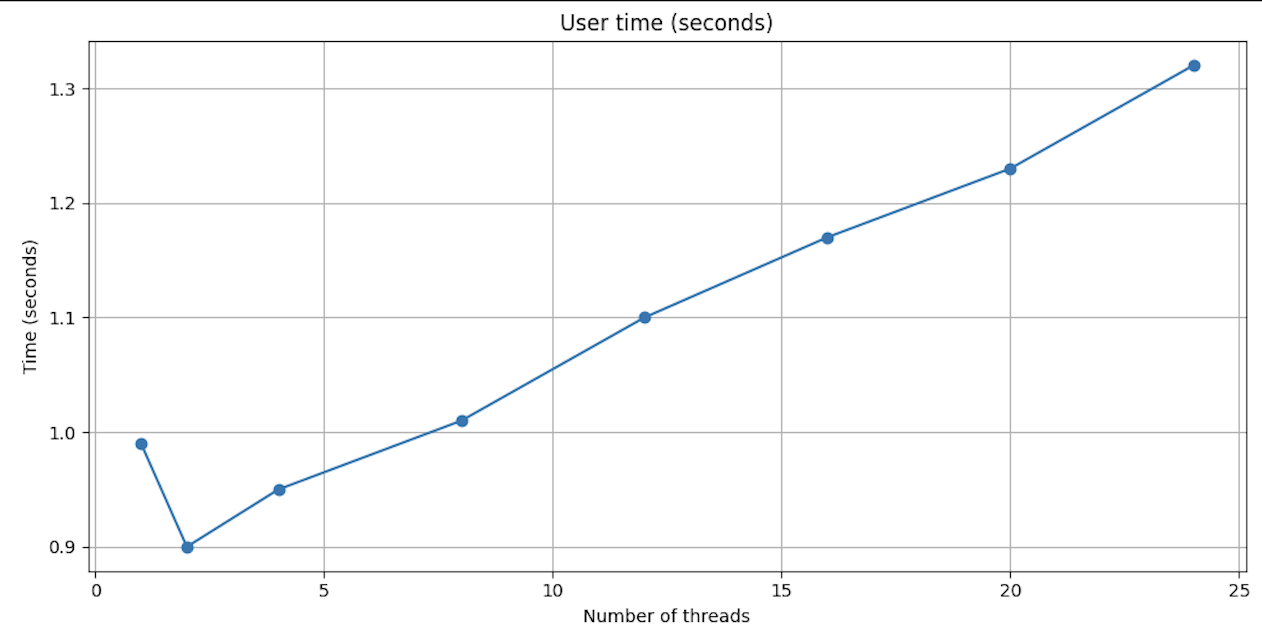
\includegraphics[width=1\linewidth]{figures/eff_omp_1.png}
\caption{OMP Efficiency Analysis}
\label{}
\end{wrapfigure}

\begin{itemize}
\tightlist
\item
  \textbf{User time}: The graph of user time shows an almost linear
  increase as the number of thread increases. This indicates that the
  program is performing more overall work with the addition of threads,
  which is to be expected if each thread performs a significant portion
  of the total work. However, a linear increase in user time with more
  threads could also suggest that there are portions of code that do not
  benefit from parallelism or that there are synchronisations or
  communication latencies that limit the effectiveness of
  parallelisation. Ideally, we would like to see a plateau or even a
  decrease in user time per thread as the number of threads increases,
  indicating an effective use of parallelism to reduce the load on each
  core.
\end{itemize}

\begin{wrapfigure}{r}{0.5\textwidth}
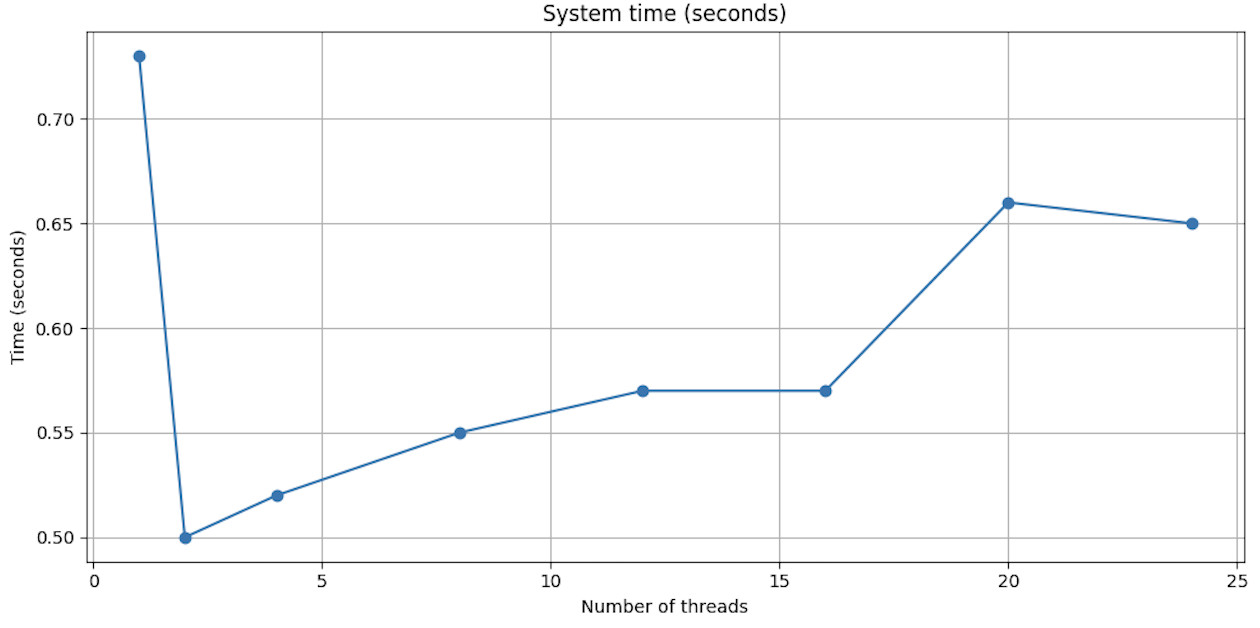
\includegraphics[width=1\linewidth]{figures/eff_omp_2.png}
\caption{OMP Efficiency Analysis}
\label{}
\end{wrapfigure}

\begin{itemize}
\tightlist
\item
  \textbf{System time}: The system tume initially shows a dramatic
  decrease, stabilising later and increasing slightly as more threads
  are added. The initial decrease is positive, indicating that the
  system overhead per thread decreases when there are few threads. The
  later increase may reflect the increasing overhead associated with
  handling more threads. An increase in system time with many threads
  may indicate that the management of the threads themselves, including
  synchronisation between them, is consuming system resources. It could
  be useful to explore methods of reducing this overhead, such as
  optimising critical sections of code or using a different parallelism
  model.
\end{itemize}

\begin{wrapfigure}{r}{0.5\textwidth}
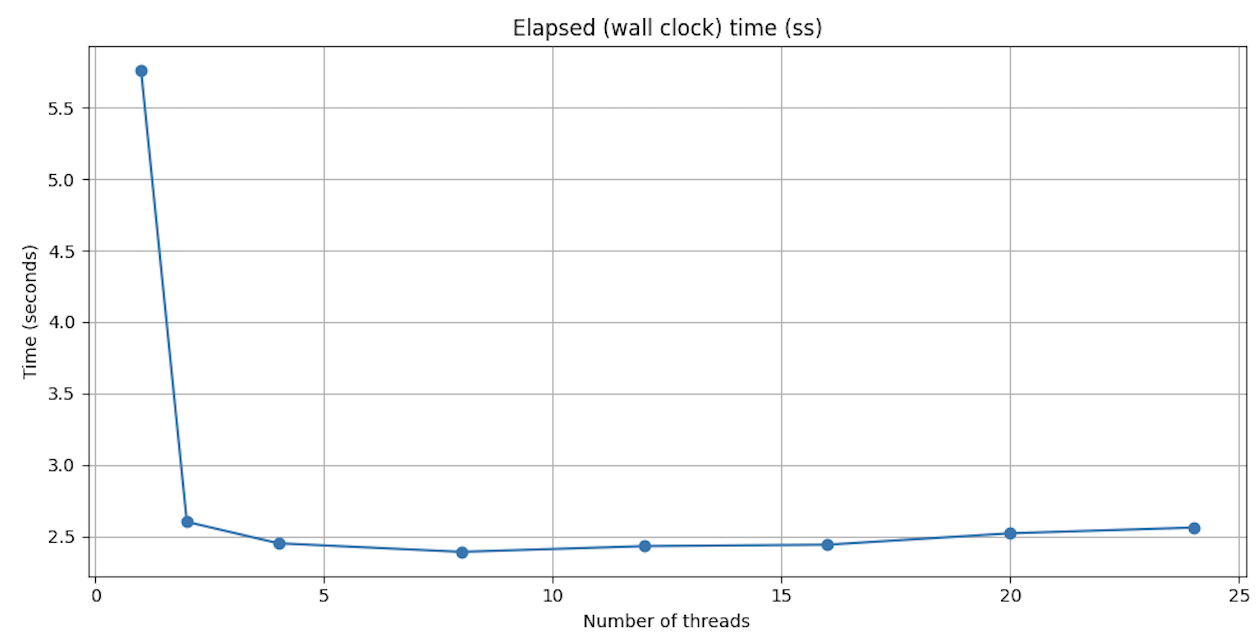
\includegraphics[width=1\linewidth]{figures/eff_omp_3.png}
\caption{OMP Efficiency Analysis}
\label{}
\end{wrapfigure}

\begin{itemize}
\tightlist
\item
  \textbf{Elapsed (wall clock) time}: This graph shows a significant
  improvement in total execution time as the number of threads increases
  from 1 to 12, after which the benefits stabilise. This is a clear
  indicator that the application benefits from parallelism up to a
  certain point, beyond which thread management overheads and resource
  saturation probably limit further improvements. The plateau in
  execution time suggests that there are physical limits or limitations
  in the code that prevent further improvements. Further optimisation of
  the code or an exploration of hardware limitations, such as memory
  bandwidth or cache conflicts, which may affect scalability, may be
  necessary.
\end{itemize}

In summary, the results show that the programme benefits from the
addition of threads up to a certain number, after which the gains in
execution time are reduced. This is typical of programmes performing
heavy calculations that can be effectively parallelised, but only as
long as no resource bottlenecks or architecture limitations are
encountered.

\begin{wrapfigure}{r}{0.5\textwidth}
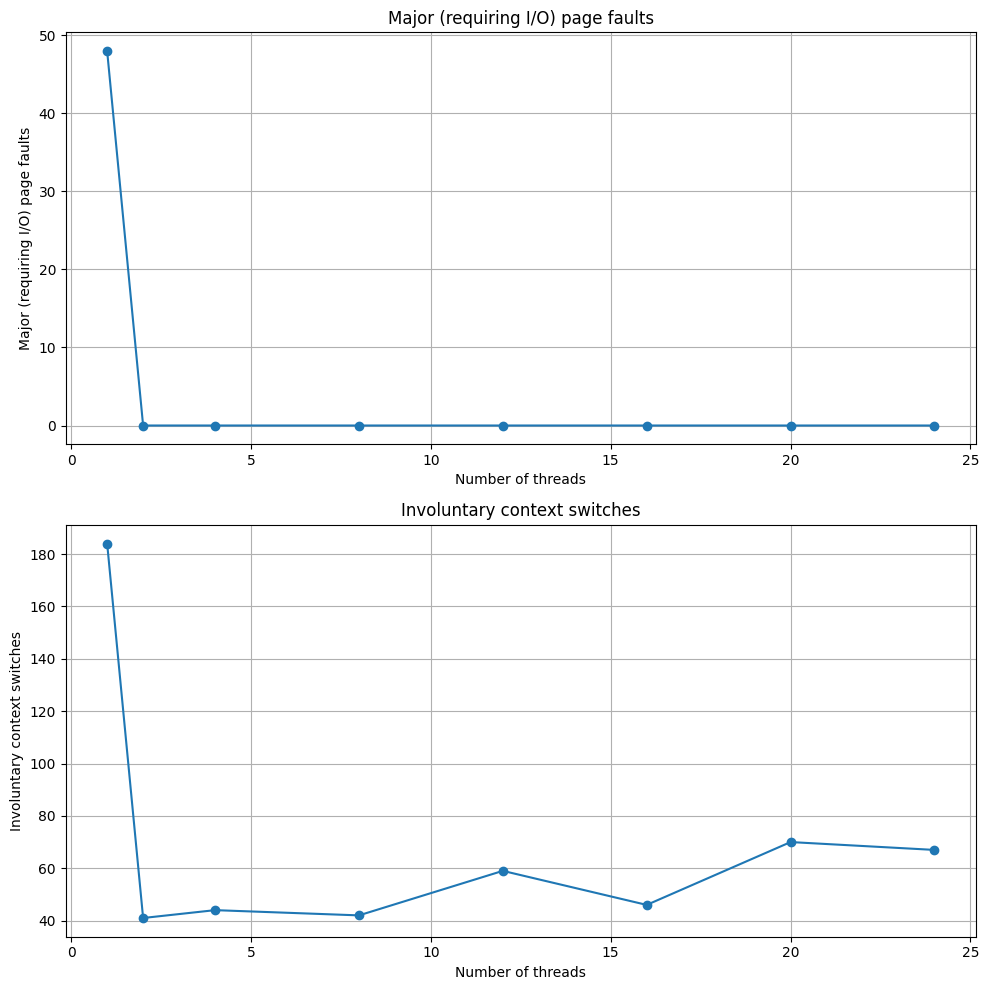
\includegraphics[width=1\linewidth]{figures/bott_omp.png}
\caption{OMP Bottlenecks Analysis}
\label{}
\end{wrapfigure}

\subsubsection{Bottlenecks}\label{bottlenecks}

\begin{itemize}
\item
  \textbf{Major (requiring I/O) page faults}: The graph of `major page
  faults' shows a high number of faults when using a single thread, with
  a drastic decrease already with the introduction of a few additional
  threads, then stabilising at zero for subsequent thread increments. A
  high major page fault at the beginning may indicate that the process
  is accessing a large amount of data for the first time, which is not
  resident in memory and must be loaded from slower storage devices
  (such as disk). The rapid decrease with multiple threads suggests that
  once data is loaded into memory, access becomes more efficient and
  less likely to cause further page faults. This may be a sign that
  memory is efficiently shared and utilised between threads after the
  first load.
\item
  \textbf{Involuntary context switches}: Involuntary context switches
  show a high frequency at the beginning with only one thread, followed
  by a marked decrease and then a slight fluctuation but generally
  remaining at lower levels. A high number of initial involuntary
  context switches may be due to the fact that the operating system
  often has to intervene to manage the process, possibly due to resource
  waits. The decrease as threads increase indicates that the workload is
  more evenly distributed among threads, reducing the need for the
  operating system to intervene frequently. Fluctuations in later stages
  may reflect competition for system resources such as CPU or memory,
  particularly when the number of threads approaches the number of
  available physical cores.
\end{itemize}

The significant decrease in both page faults and involuntary context
switches as threads increase is positive, indicating that the programme
scales well in terms of resource management as parallelism increases.
However, it is also essential to monitor these metrics to assess whether
other types of overhead or limitations occur, such as memory bandwidth
saturation or cache limitations, which may not be immediately apparent
from execution times alone.

\begin{wrapfigure}{r}{0.5\textwidth}
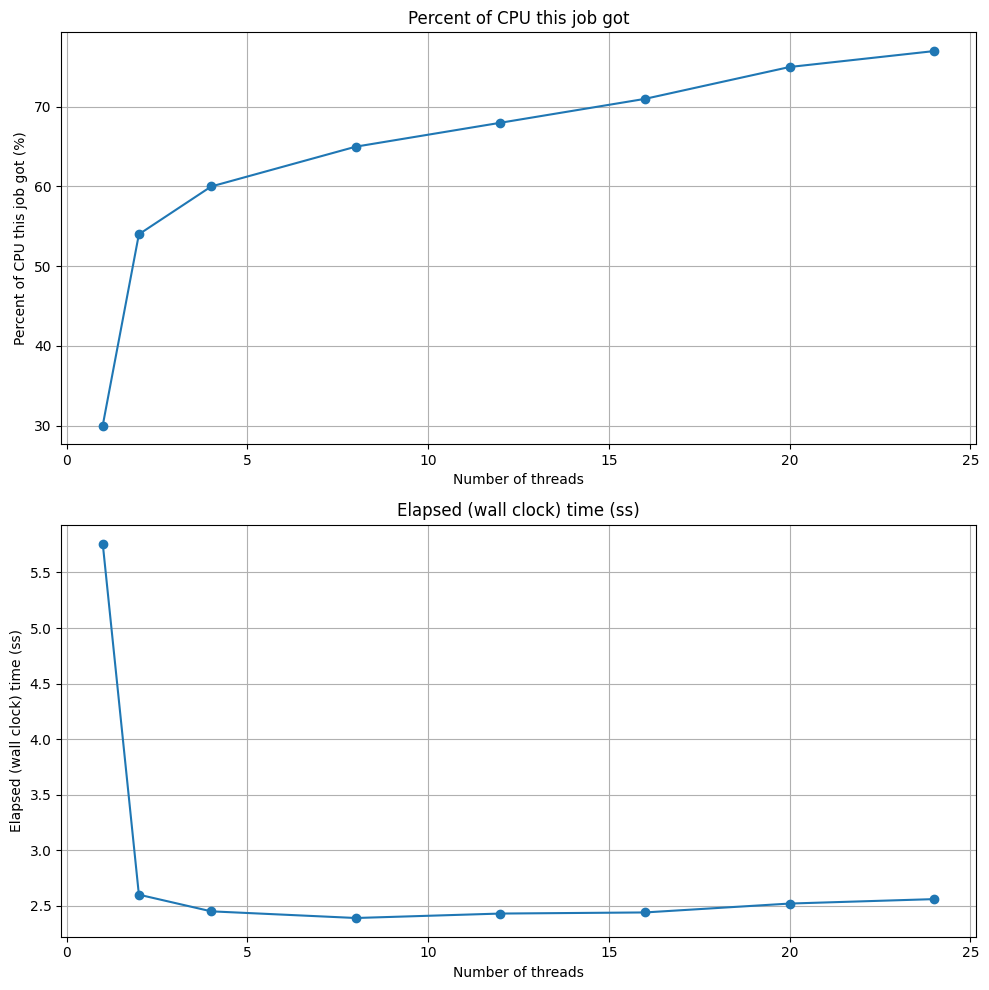
\includegraphics[width=1\linewidth]{figures/par_omp.png}
\caption{OMP Parallelisation Impact Analysis}
\label{}
\end{wrapfigure}

\subsubsection{Parallelisation Impact}\label{parallelisation-impact}

\begin{itemize}
\item
  \textbf{Percent of CPU this job got}: This graph shows a marked
  increase in the percentage of CPU used as the number of threads
  increases, starting from a relatively low level with only one thread
  and rising consistently to a plateau around 70 per cent. The increase
  in CPU percentage indicates that adding more threads allows the
  programme to utilise more processor resources simultaneously,
  suggesting good initial scalability of parallelism. The plateau may
  indicate that the programme is reaching the limits of scalability on
  this particular hardware architecture, possibly due to physical
  limitations such as the number of available cores, memory bandwidth
  saturation, or the workload is no longer able to be effectively
  divided between additional threads.
\item
  \textbf{Elapsed (wall clock) Time}: The graph of execution time shows
  a sharp drop in execution time when going from 1 to several threads,
  then stabilising at a low value after about 4 threads. This is a
  typical indicator of a good response to initial parallelisation. The
  rapid reduction in execution time as the first threads increase shows
  that the programme benefits significantly from the distribution of the
  workload among multiple threads.
\end{itemize}

These results indicate that the programme has a good degree of
parallelism up to a certain number of threads, beyond which no
significant benefits are achieved. This type of information is crucial
for deciding how to allocate resources in a production environment and
for optimising further software development:

\begin{itemize}
\tightlist
\item
  Optimising the Number of Threads: Based on the results, it may be
  ideal to configure the programme to use a number of threads close to
  the plateau point to maximise efficiency.
\item
  Exploration of Other Optimisations: Consider exploring optimisations
  beyond simply increasing the number of threads, such as improvements
  in the algorithm, memory management and synchronisation overhead
  reduction.
\end{itemize}

\subsection{MPI Analysis}\label{mpi-analysis}

The script was run with a single OpenMP thread per MPI task and
increasing the number of MPI tasks. For this test was requested 2 nodes,
using all the cores available on the THIN nodes.

\begin{verbatim}
## Load the required modules
module load openMPI/4.1.5/gnu/12.2.1

## Compile the program
mpicc -o mandelbrot_scal_mpi -fopenmp mandelbrot_mpi_omp.c

## Number of processes MPI to test for scalability
num_procs=(1 2 4 8 16 24 36 48)

## Run the program in loop for each number of processes
for procs in "${num_procs[@]}"
do
    echo "Running with ${procs} processes:"
    /usr/bin/time -v mpirun -np ${procs} ./mandelbrot_scal_mpi
done

echo "Scalability test is complete."
\end{verbatim}

\subsubsection{Efficiency}\label{efficiency-1}

\begin{figure}
\centering
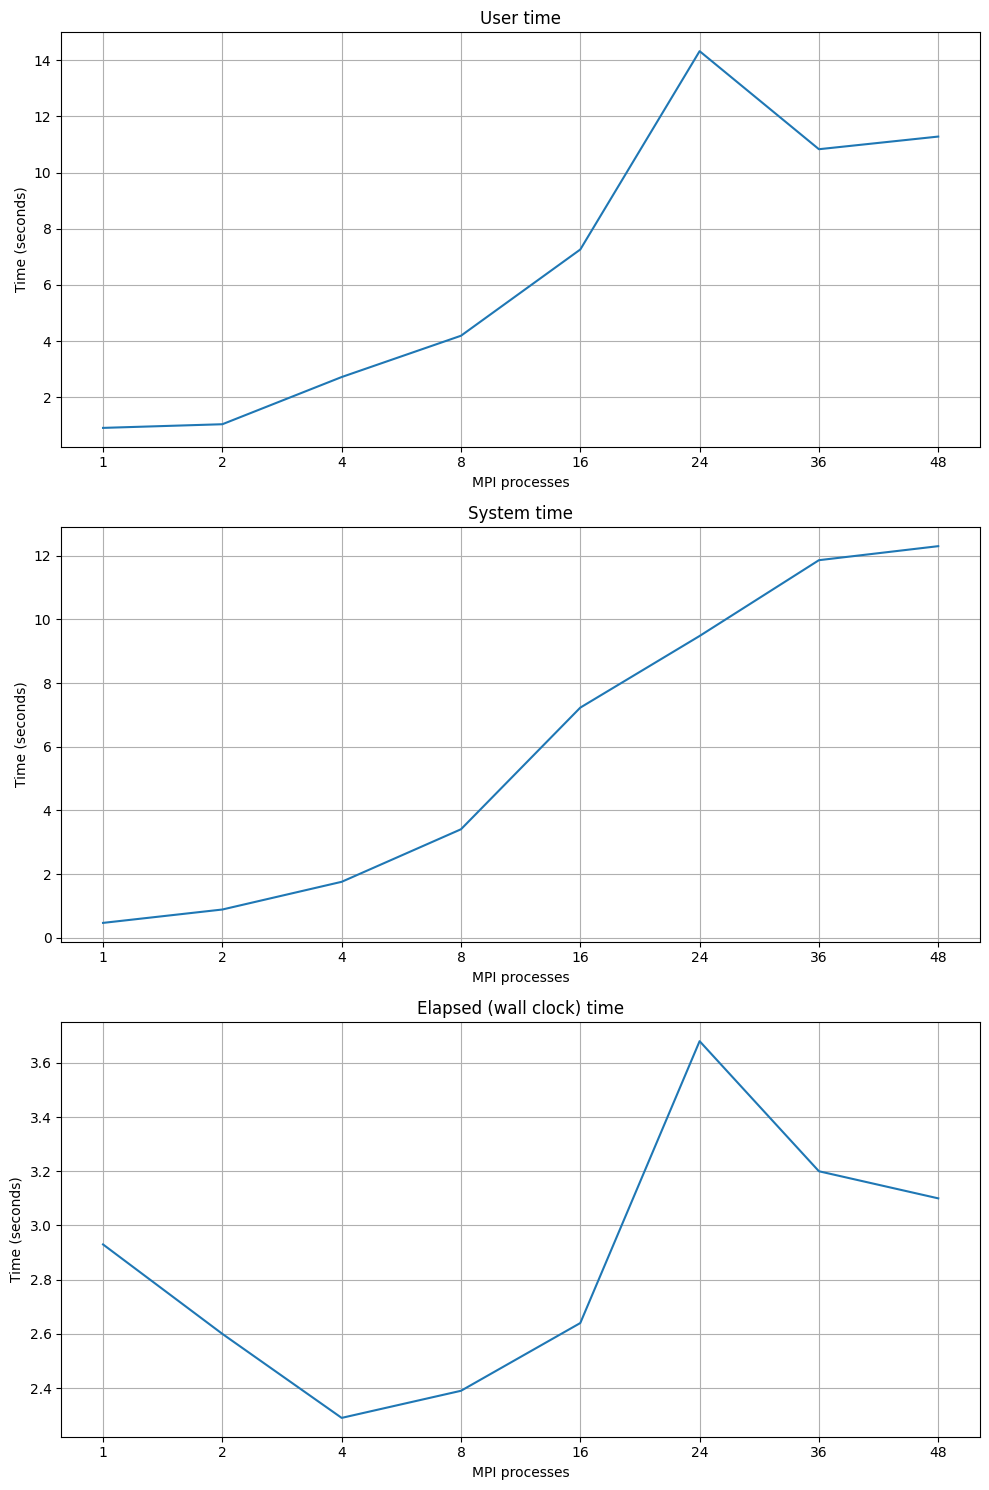
\includegraphics{figures/eff_mpi.png}
\caption{MPI Efficiency}
\end{figure}

\begin{itemize}
\item
  \textbf{User time}: The curve shows an increase up to 16 processes,
  then a peak at 24 processes before decreasing and finally increasing
  again with 48 processes. The increase in user time to 16 processes may
  indicate that the addition of MPI processes does indeed contribute to
  the computational workload. However, the spike to 24 processes and
  subsequent decrease may suggest inefficiencies, possibly due to
  communication congestion or sub-optimal workload distribution.
\item
  \textbf{System time}: The steady increase in system time with the
  increase in MPI processes suggests that there is an increasing system
  overhead, which may include handling communication between processes.
  The constant increase is an indicator that more processes result in
  higher communication or synchronisation costs at system level, which
  are not compensated for by a proportional increase in computing speed,
  leading to a decrease in overall efficiency.
\item
  \textbf{Elapsed (wall clock) time}: The graph initially shows a
  decreasing trend up to 4 processes, indicating good scalability.
  However, the time increases sharply at 16 processes, then increases
  dramatically at 24 before dropping to 48. The trend in execution time
  shows that there are peaks of inefficiency, especially at 24
  processes. This could be due to increased waiting time for resources
  or inefficient handling of inter-process communication.
\end{itemize}

Overall, the scalability of the programme does not appear linear and
shows signs of communication and system management overheads that affect
overall efficiency as the number of processes increases. This could be
due the nature of the problem, lack of load balancing between processes,
congestion in the network or communications, or inefficient utilisation
of system resources due to the configuration of the computing topology.

\subsubsection{Bottlenecks}\label{bottlenecks-1}

\begin{figure}
\centering
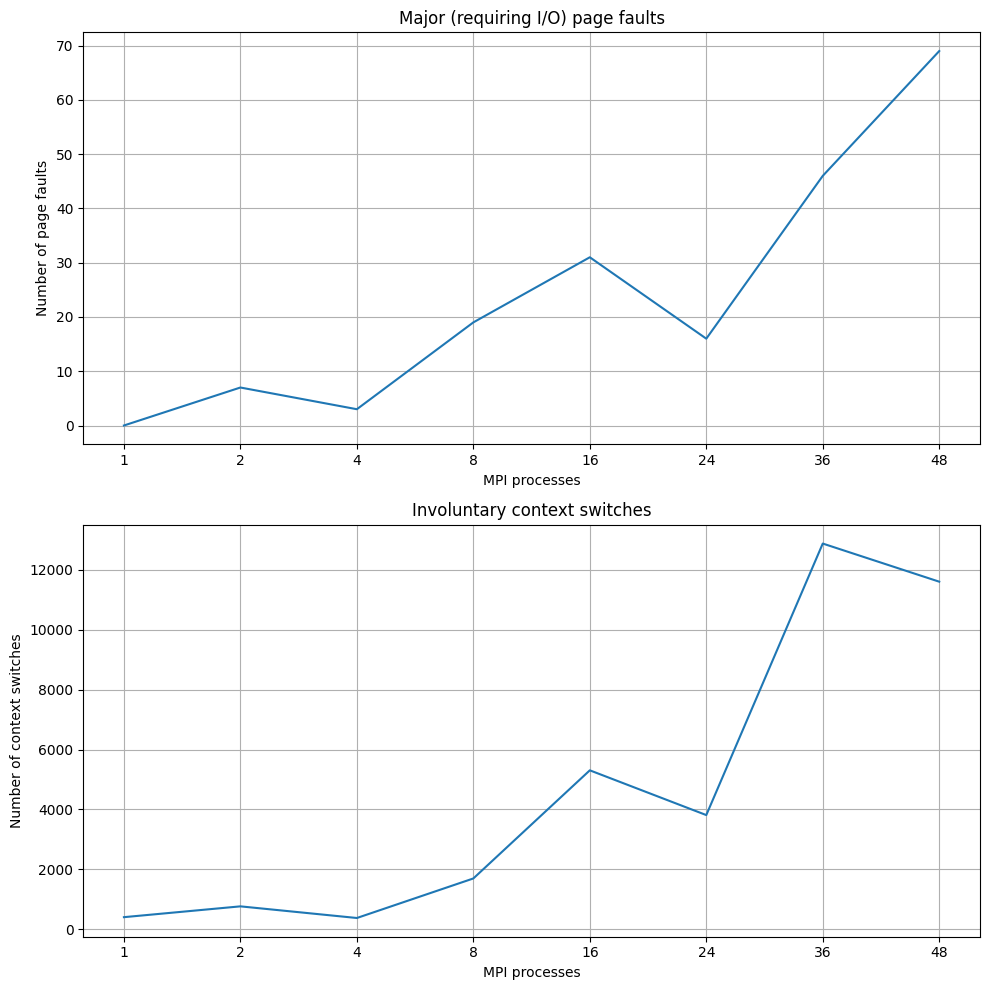
\includegraphics{figures/bott_mpi.png}
\caption{MPI Bottlenecks}
\end{figure}

\begin{itemize}
\item
  \textbf{Major (requiring I/O) page faults}: Major page faults occur
  when the system has to read a page of memory from the disk because it
  is not present in RAM. This can happen if the process requires more
  memory than is physically available, forcing the system to swap pages
  between RAM and disk. The number of `Major page faults' increases as
  the number of MPI processes increases, showing a significant peak at
  16 processes, a decrease at 24, and then a further sharp increase to
  48. This suggests that the system may be under memory pressure as the
  number of processes increases, forcing the operating system to resort
  to I/O operations that are significantly slower than memory
  operations.
\item
  \textbf{Involuntary context switches}: The number of `Involuntary
  context switches' initially increases as the number of processes
  increases, shows a peak at 16 processes, then decreases to 24, and
  increases dramatically to 36 before decreasing again to 48. This
  indicates that there are potential inefficiencies in process
  management and CPU scheduling, especially with a large number of
  processes.
\end{itemize}

The increasing frequency of `major page faults' suggests that it might
be worth optimising memory usage within the programme. High `Involuntary
context switches' indicate that the workload may not be distributed
efficiently among processes, or that the waiting time for resources
(such as memory or I/O) is adversely affecting performance.

\subsubsection{Parallelisation Impact}\label{parallelisation-impact-1}

\begin{figure}
\centering
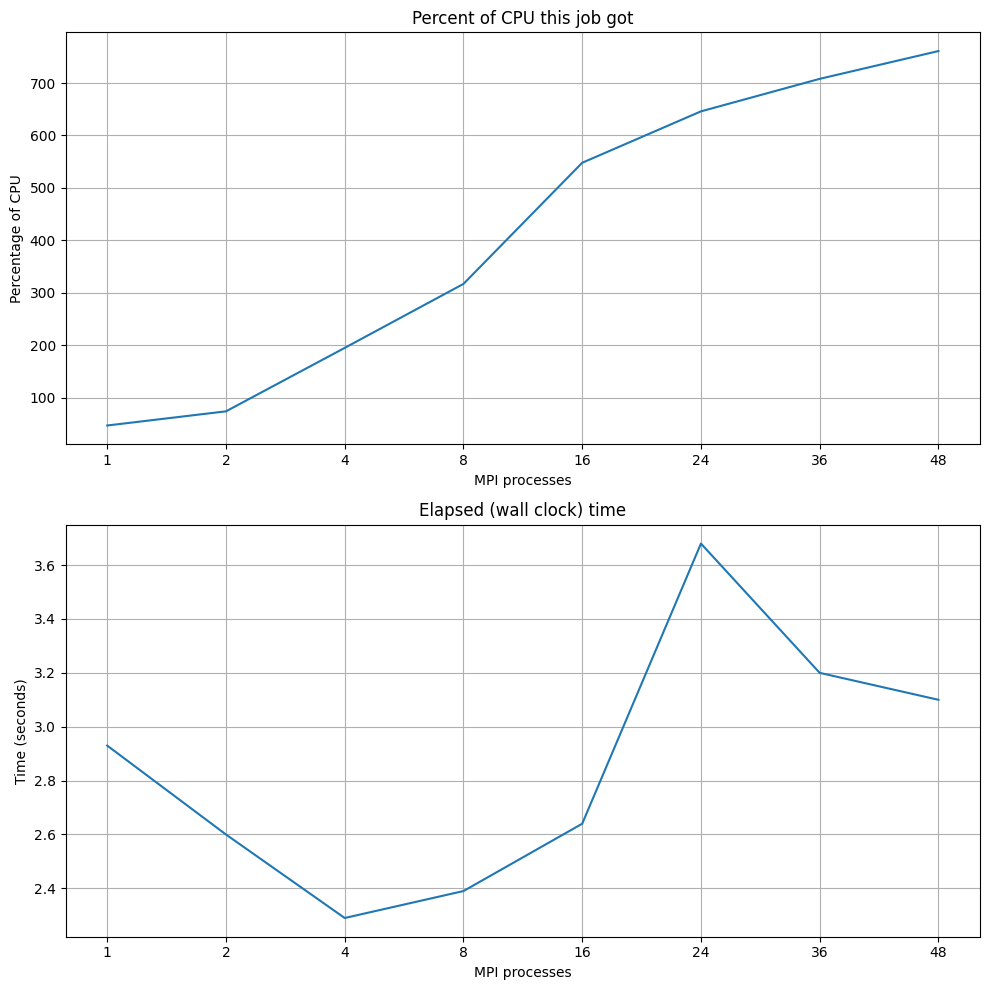
\includegraphics{figures/par_mpi.png}
\caption{MPI Parallelisation Impact}
\end{figure}

\begin{itemize}
\item
  \textbf{Percent of CPU this job got}: The percentage of CPU
  utilisation increases almost linearly with the increase in the number
  of MPI processes, indicating that the increase in processes leads to
  higher overall CPU utilisation. This is a positive sign suggesting
  good scalability in terms of the ability to handle parallel workloads.
  However, an increase above 100 per cent indicates that several cores
  are being used simultaneously, which is expected in a parallel
  environment such as MPI on a multicore system.
\item
  \textbf{Elapsed (wall clock) Time}: This graph shows the total elapsed
  time from the beginning to the end of programme execution, which is
  essential for assessing the effectiveness of parallelisation in terms
  of reducing execution time. The trend shows a significant improvement
  in execution time as the number of processes increases from 1 to 8,
  indicating that parallelisation is having a positive impact. However,
  there is an unexpected peak at 24 processes, followed by a drop to 36
  before a reduction to 48.
\end{itemize}

Analyses indicate that the programme benefits from parallelisation up to
a certain number of processes, beyond which gains are reduced due to
management overhead and communication complexity. These results suggest
that there are key areas that can be optimised to further improve
performance, such as memory management, workload balancing, minimising
communication overheads and synchronisation.

\subsection{Hybrid Analysis}\label{hybrid-analysis}

In this extra analysis, it was run the script with different
combinations of MPI and OpenMP threads to analyse the scalability of the
hybrid implementation. The script was run with a varying number of MPI
tasks and OpenMP threads per task. For this test was requested 2 nodes,
using half of the cores available on the THIN nodes.

\begin{verbatim}
## Compile the program
mpicc -o mandelbrot_hybrid -fopenmp mandelbrot_mpi_omp.c

## Executing the program with different number of MPI processes and OpenMP threads
for procs in 2 4 8 16 24
do
   for threads in 1 2 4 8 12
   do
      export OMP_NUM_THREADS=$threads
      echo "Running with $procs MPI processes and $threads OpenMP threads:"
      /usr/bin/time -v mpirun -np $procs ./mandelbrot_hybrid
   done
done
\end{verbatim}

\subsubsection{Efficiency}\label{efficiency-2}

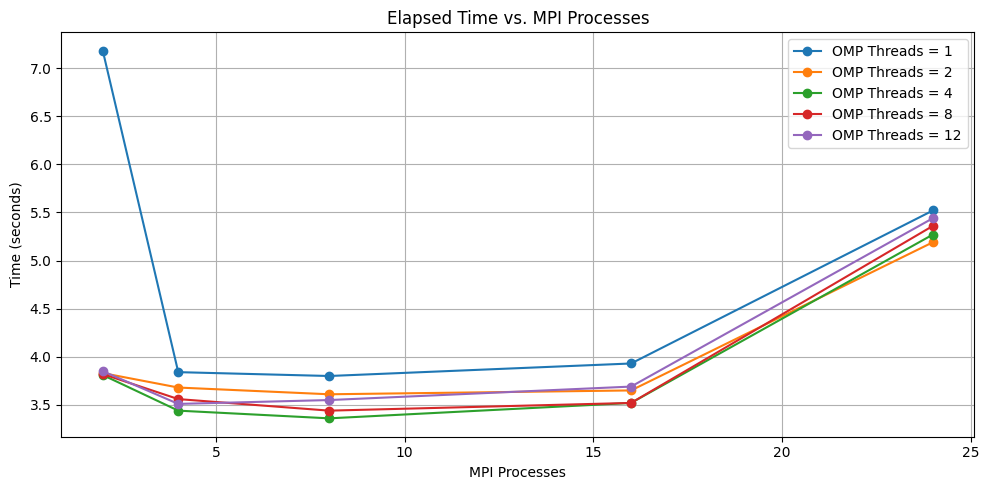
\includegraphics{figures/elapsed_time.png}
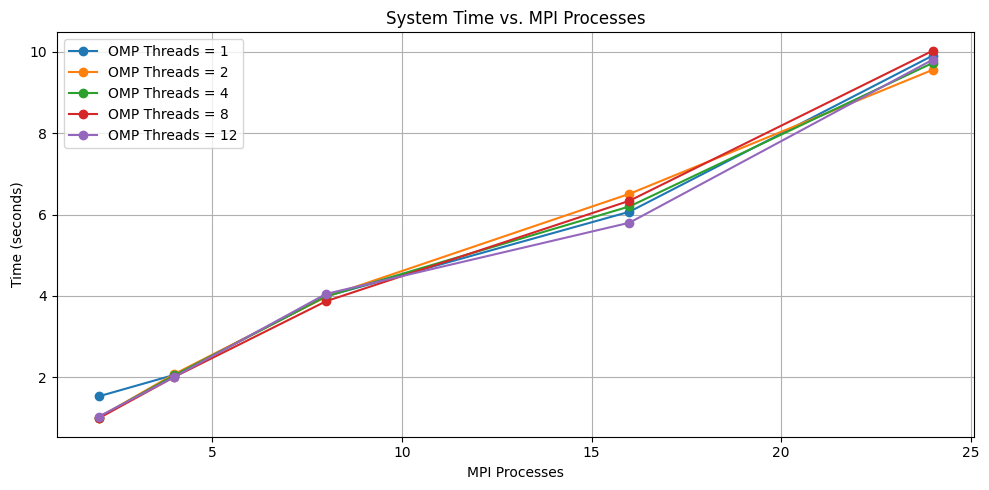
\includegraphics{figures/system_time.png}
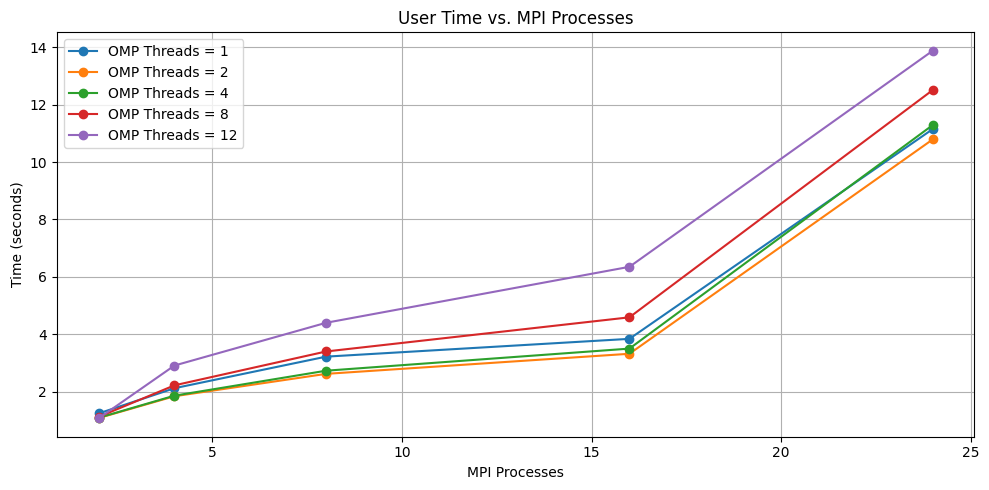
\includegraphics{figures/user_time.png}

\begin{itemize}
\item
  \textbf{Scalability}: The decrease in elapsed time from 2 to 4 MPI
  processes shows initial scalability. However, beyond 4 MPI processes,
  the performance gains are less clear, and in some cases, the elapsed
  time increases. The system time increases linearly, indicating that
  the computational overhead scales proportionally with more MPI
  processes.
\item
  \textbf{Threading Efficiency}: Higher OpenMP thread counts (8 and 12)
  show significantly higher user times, which might indicate
  inefficiencies or overhead in managing a large number of threads. For
  lower MPI process counts, using more OpenMP threads seems to improve
  elapsed time, but this benefit diminishes as the number of MPI
  processes increases.
\item
  \textbf{Optimal Configuration}: For the given setup, using around 4
  MPI processes with moderate OpenMP threads (4-8) seems to provide a
  good balance between user time, system time, and elapsed time. Using
  too many OpenMP threads (12) significantly increases user time, which
  suggests diminishing returns or potential bottlenecks in threading.
\end{itemize}

\subsubsection{Bottlenecks}\label{bottlenecks-2}

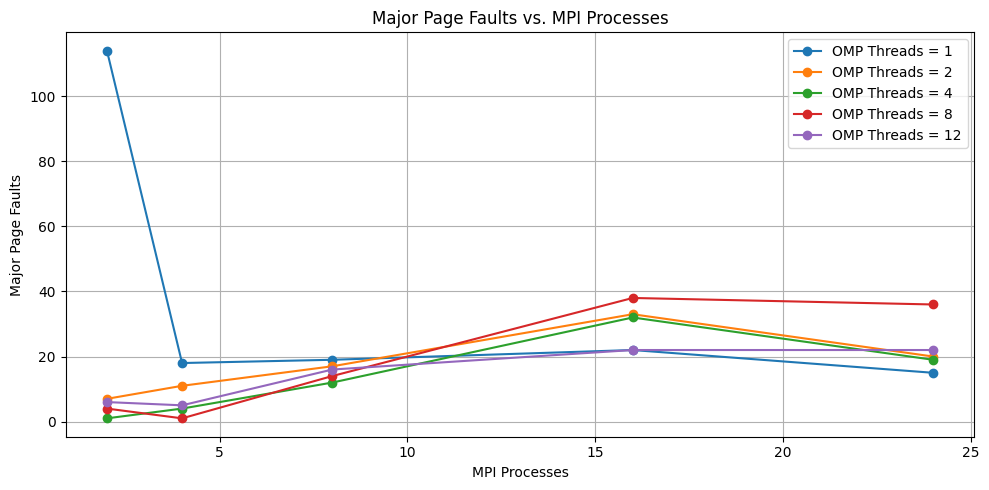
\includegraphics{figures/major_page.png}
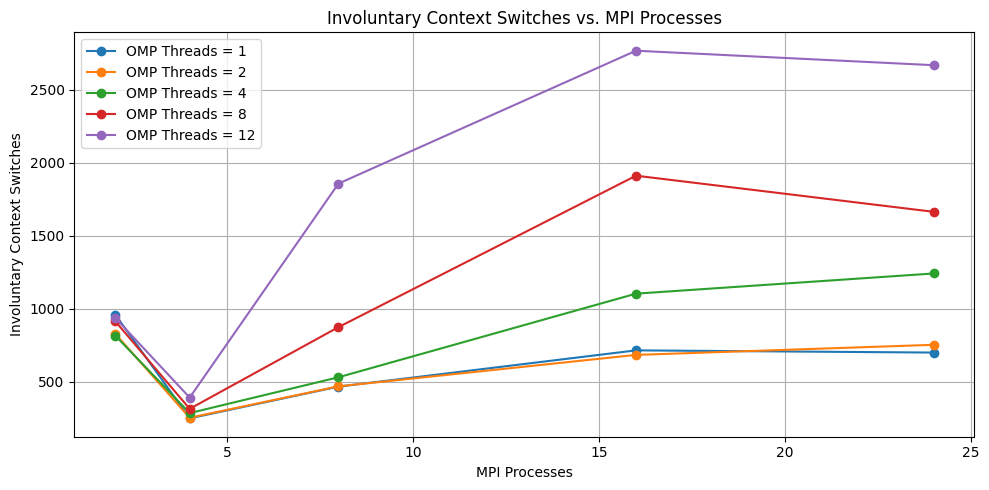
\includegraphics{figures/inv_cont.png}

\begin{itemize}
\item
  \textbf{Context Switch Overhead}: The increase in involuntary context
  switches with higher OpenMP threads suggests significant overhead in
  managing threads, particularly for configurations with many MPI
  processes. This could be due to thread contention, synchronization
  issues, or inefficient scheduling.
\item
  \textbf{Memory Access Issues}: The initial high number of major page
  faults for 1 OpenMP thread with 2 MPI processes may indicate memory
  access patterns that cause significant paging. However, this issue
  diminishes with more processes and threads. For higher OpenMP thread
  counts, the increased page faults suggest potential memory contention
  or inefficient use of shared memory resources.
\item
  \textbf{Optimal Configuration}: To minimize context switches and page
  faults, a balanced configuration with moderate MPI processes and
  OpenMP threads (e.g., 4-8 threads) appears optimal. Avoid
  configurations with excessively high thread counts (e.g., 12 threads)
  as they introduce significant overhead and inefficiencies.
\end{itemize}

\subsubsection{Parallelisation Impact}\label{parallelisation-impact-2}

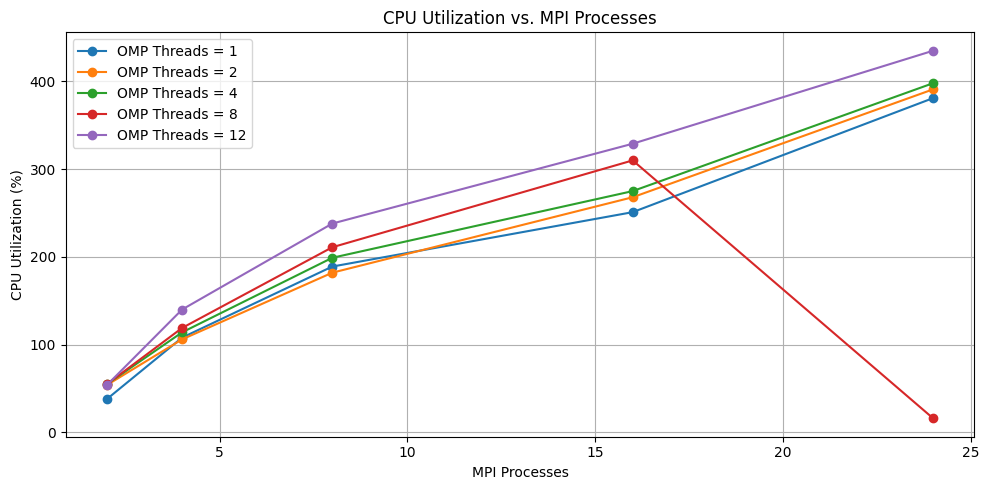
\includegraphics{figures/cpu.png} 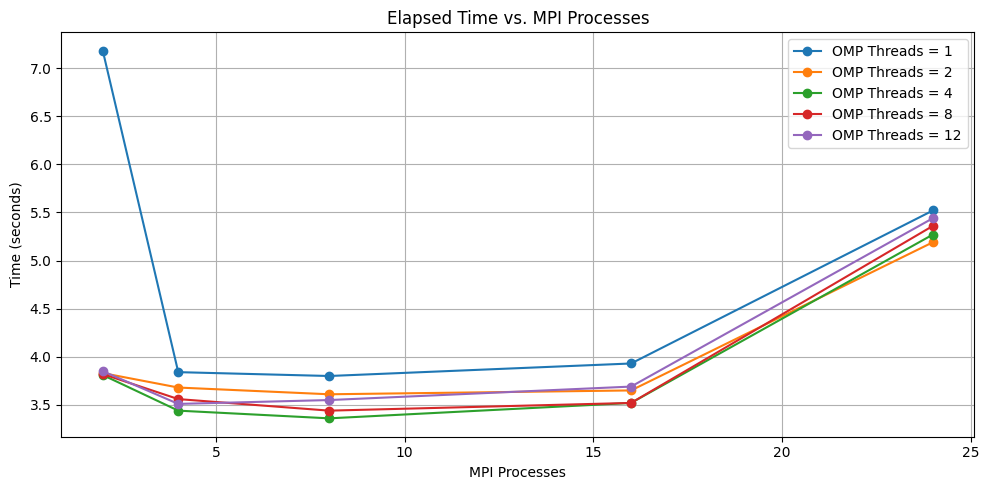
\includegraphics{figures/elapsed.png}

\begin{itemize}
\item
  \textbf{Scalability and Efficiency}: The initial decrease in elapsed
  time from 2 to 4 MPI processes shows good scalability and parallel
  efficiency. Beyond 4 MPI processes, the benefits of additional
  processes diminish, and the system might be hitting resource
  contention or communication overheads, especially evident at 24 MPI
  processes.
\item
  \textbf{Threading Efficiency}: Higher OpenMP thread counts (8 and 12)
  improve CPU utilization, indicating better use of multicore resources.
  The anomaly observed with 8 OpenMP threads at 24 MPI processes
  suggests there might be specific issues with this configuration,
  potentially due to over-subscription or inefficiencies in thread
  management.
\item
  \textbf{Optimal Configuration}: The best performance in terms of
  minimizing elapsed time and maximizing CPU utilization seems to be
  around 4-8 MPI processes with 4-8 OpenMP threads. Extremely high
  thread counts (12) can lead to higher CPU utilization but also
  increased overheads, affecting user time and system time negatively.
\end{itemize}

\subsection{Conclusion}\label{conclusion}

This investigation into the scalability of the Mandelbrot set
computation using a hybrid MPI and OpenMP setup reveals several key
insights into efficiency, bottlenecks, and parallelization impact.

\subsubsection{Efficiency}\label{efficiency-3}

The efficiency analysis shows that user time, system time, and elapsed
time are crucial metrics. User time tends to increase with the number of
MPI processes, with a significant rise when using higher OpenMP thread
counts, particularly at 12 threads. System time increases linearly with
MPI processes, indicating a proportional computational overhead. Elapsed
time decreases significantly when moving from 2 to 4 MPI processes,
demonstrating good initial scalability. However, beyond 4 MPI processes,
the benefits diminish, and elapsed time either stabilises or slightly
increases. The optimal configuration for efficiency is around 4-8 MPI
processes with 4-8 OpenMP threads, avoiding configurations with 12
threads due to increased overhead.

\subsubsection{Bottlenecks}\label{bottlenecks-3}

The bottleneck analysis focuses on major page faults and involuntary
context switches. Involuntary context switches increase with the number
of MPI processes, especially at higher OpenMP thread counts, indicating
thread management overhead. Major page faults are initially high with 1
thread and 2 MPI processes but stabilize with higher process counts.
Configurations with higher thread counts tend to have more page faults,
suggesting memory contention or inefficiencies. Minimizing bottlenecks
involves using moderate MPI processes (4-8) and OpenMP threads (4-8),
avoiding the overhead introduced by high thread counts.

\subsubsection{Parallelization Impact}\label{parallelization-impact}

The parallelization impact is assessed through CPU utilization and
elapsed time. CPU utilization increases with MPI processes and higher
OpenMP thread counts, indicating effective use of multicore resources.
An anomaly with 8 OpenMP threads at 24 MPI processes shows a significant
drop in CPU utilization, suggesting resource contention or
inefficiencies at higher concurrency levels. Elapsed time decreases
significantly from 2 to 4 MPI processes, demonstrating good scalability,
but stabilizes or increases slightly beyond this point. Lower thread
counts (1-2) result in higher elapsed times compared to higher counts
(4-12).

\subsubsection{Optimal Configuration and
Recommendations}\label{optimal-configuration-and-recommendations}

The best performance for the Mandelbrot set computation is achieved with
4-8 MPI processes and 4-8 OpenMP threads. Extremely high thread counts
(12) lead to higher CPU utilization but also increased overheads,
negatively impacting efficiency. Things that could be consiered to
further optimize performance:

\begin{itemize}
\tightlist
\item
  Investigating and optimizing thread management to reduce user time and
  context switches at high thread counts.
\item
  Optimize memory access patterns to reduce major page faults and
  improve overall efficiency.
\item
  Conduct additional tests with configurations around 4-8 MPI processes
  and 4-8 OpenMP threads to refine the optimal setup.
\item
  Use profiling tools to identify and optimize specific functions or
  operations causing inefficiencies.
\end{itemize}

\end{document}
